\section{实验设置}
\label{sec:exp}

\begin{table*}[t]
    \footnotesize
    \centering
    \rowcolors{1}{white}{gray!10}
    \caption{\textbf{性能优先设置下 LoCoMo、LongMemEval 和 HotpotQA 的实验结果，指标包括 F1 分数（F1）、LLM 评审（Judge）和成本。}}
    \label{tab:exp_main}
    \begin{tabular}{lcccccccccccc}
        \toprule
        \rowcolor{white}
        \textbf{方法} &
        \multicolumn{3}{c}{\textbf{LoCoMo}} &
        \multicolumn{3}{c}{\textbf{LongMemEval}} &
        \multicolumn{3}{c}{\textbf{HotpotQA}} &
        \multicolumn{3}{c}{\makecell[c]{\rowcolor{white}\textbf{平均}}} \\
        \cmidrule(lr){2-4} \cmidrule(lr){5-7} \cmidrule(lr){8-10} \cmidrule(lr){11-13}
        \rowcolor{white}
        & \textbf{F1} & \makecell[c]{\rowcolor{white}\textbf{评审}} & \textbf{成本$^\downarrow$}
        & \textbf{F1} & \makecell[c]{\rowcolor{white}\textbf{评审}} & \textbf{成本$^\downarrow$}
        & \textbf{F1} & \makecell[c]{\rowcolor{white}\textbf{评审}} & \textbf{成本$^\downarrow$}
        & \textbf{F1} & \makecell[c]{\rowcolor{white}\textbf{评审}} & \textbf{成本$^\downarrow$} \\
        \midrule
        \rowcolor{white}
        \multicolumn{13}{l}{\textbf{LLaMA-3.3-70B-Instruct}} \\
        ReadAgent & 22.48 & 31.05 & 0.57 & 20.75 & 27.72 & 13.68 & 15.33 & 30.08 & 4.19 & 19.52 & 29.62& 6.14 \\
        MemoryBank & 22.27 & 28.98 & 0.73 & 26.74 & 32.67 & 3.94 & 22.25 & 23.75 & 7.75 & 23.75 & 28.47 & 4.14 \\
        A-MEM & 26.43 & 32.96 & 2.88 & 21.74 & 33.17 & 80.02 & 43.25 & 54.69 & 26.74 & 30.47 & 40.27 & 32.07 \\
        LangMem & 22.31 & 25.96 & \textbf{0.48} & 12.00 & 17.00 & 16.60 & 22.78 & 22.66 & 10.95 & 19.03 & 21.87 & 9.34 \\
        Mem0 & 11.04 & 28.18 & 2.89 & 27.70 & 42.08 & 13.57 & 28.03 & 36.72& 4.30 & 22.26 & 35.66 & 6.92 \\
        MemoryOS & 30.62 & 34.55 & 1.97 & 12.97 & 33.50 & 38.83 & 34.50 & 43.36 & 13.32 & 26.03 & 37.14 & 18.04 \\
        LightMem & 33.88 & 40.76 & 1.50 & 26.74 & 48.51 &  5.28 & 45.73 & 58.37 & 10.10 & 35.45 & 49.21 & 5.63 \\
        \midrule
        \rowcolor{row-highlight}\textbf{BudgetMem-\textsc{Imp}} &
        38.75 & 50.32 & 1.80 &
        37.47 & 56.00 & 0.71 &
        49.31 & \textbf{65.77} & 1.35 &
        41.84 & 57.36 & \textbf{1.29} \\
        \rowcolor{row-highlight}\textbf{BudgetMem-\textsc{Rea}} &
        40.92 & 52.23 & 2.90 &
        \textbf{40.53} & 58.00 & \textbf{0.67} &
        51.12 & 61.93 & 0.99 &
        44.19 & 57.39 & 1.52 \\
        \rowcolor{row-highlight}\textbf{BudgetMem-\textsc{Cap}} &
        \textbf{43.05} & \textbf{54.62} & 2.40 &
        40.24 & \textbf{60.50} & 0.80 &
        \textbf{53.87} & 64.85 & \textbf{0.93} &
        \textbf{45.72} & \textbf{59.99} & 1.38 \\
        \midrule
        \rowcolor{white}
        \multicolumn{13}{l}{\textbf{Qwen3-Next-80B-A3B-Instruct}$^\dagger$} \\
        ReadAgent & 22.45 & 31.37 & 0.24 & 27.72 & 20.75 & 4.97 & 18.05 & 25.78 & 1.75 & 22.74 & 25.97& 2.32 \\
        MemoryBank & 23.53 & 34.71 & 0.25 & 10.56 & 28.22 & 3.45 & 18.64 & 31.25 & 1.79 & 17.58 & 31.39 & 1.83 \\
        A-MEM & 27.65 & 38.54 & 2.88 & 10.82 & 31.19 & 21.00 & 40.54 & 50.39 & 8.34 & 26.34& 40.04& 10.74\\
        LangMem & 20.89 & 23.40 & \textbf{0.14} & 11.01 & 14.00 & 3.99 & 20.77 & 21.09 & 17.56 & 17.56 & 19.50 & 2.82 \\
        Mem0 & 10.77 & 25.32 & 1.15 & 25.71 & 36.14 & 4.96 & 24.72 & 37.89 & 2.02 & 20.40 & 33.12 & 2.71 \\
        MemoryOS & 35.43 & 38.85 & 0.75 & 13.35 & 33.00 & 15.84 & 41.21 & 53.52 & 11.68 & 30.00 & 41.79 & 9.42 \\
        LightMem & 32.85 & 42.83 & 0.70 & 27.70 & 47.52 & 3.39 & 41.29 & 55.42 & 8.56& 33.95 & 48.59 & 4.21 \\
        \midrule
        \rowcolor{row-highlight}\textbf{BudgetMem-\textsc{Imp}} &
        40.14 & \textbf{54.38} & 0.80 &
        29.18 & 52.00 & 0.30 &
        46.67 & 57.42 & 0.63 &
        38.66 & 54.60 & 0.58 \\
        \rowcolor{row-highlight}\textbf{BudgetMem-\textsc{Rea}} &
        40.19 & 53.34 & 1.11 &
        \textbf{35.84} & \textbf{59.00} & 0.26 &
        57.67 & 70.83 & \textbf{0.17} &
        \textbf{44.57} & \textbf{61.06} & 0.51 \\
        \rowcolor{row-highlight}\textbf{BudgetMem-\textsc{Cap}} &
        \textbf{41.22} & 53.18 & 0.61 &
        31.01 & 56.00 & \textbf{0.17} &
        \textbf{58.70} & \textbf{72.08} & 0.22 &
        43.64 & 60.42 & \textbf{0.33} \\
        \bottomrule
        \rowcolor{white}\multicolumn{13}{l}{\small \textbf{粗体}表示每个基础模型分组中的最佳分数；“平均”为各指标在不同数据集上的均值。} \\
        \rowcolor{white}\multicolumn{13}{l}{
        \textbf{成本}通过汇总所有模型调用的词元，并采用相应模型的输入与输出词元价格计算。}\\
        \rowcolor{white}\multicolumn{13}{l}{\small $^\dagger$ 表示未使用该基础模型训练，仅进行迁移评估。} \\
    \end{tabular}
\end{table*}


\subsection{数据集、指标与基线}
\label{sec:datasets_metrics_baselines}

\paragraph{数据集。}
我们在三个强调长程记忆与长上下文问答（QA）的基准上评估 BudgetMem：广泛用于智能体记忆评估的 \textbf{LoCoMo}~\citep{maharana2024evaluating-locomo} 和 \textbf{LongMemEval}~\citep{wu2024longmemeval}，以及作为代表性长上下文问答任务的 \textbf{HotpotQA}~\citep{yang2018hotpotqa}\footnote{我们遵循既有工作~\citep{yu2025memagent}采用的评估协议。}。

\paragraph{指标。}
我们同时报告任务性能与成本，以刻画性能--成本权衡。
任务性能方面，我们使用 F1 分数（F1）与 LLM 评审（Judge），衡量模型预测相对于真实答案的正确性。
成本方面，我们汇总 BudgetMem 在抽取期间所有模型调用的 API 用量（输入和输出词元），并依据相应服务价格把词元数量换算为货币成本，从而度量记忆抽取成本\footnote{\url{https://www.together.ai/pricing}}。

\paragraph{基线。}
我们将 BudgetMem 与一组多样且强大的记忆增强基线进行比较：
（1）\textbf{ReadAgent}~\citep{lee2024human}；（2）\textbf{MemoryBank}~\citep{zhong2024memorybank}；（3）\textbf{A-MEM}~\citep{xu2025mem}；（4）\textbf{LangMem}~\citep{LangMem}；（5）\textbf{Mem0}~\citep{chhikara2025mem0}；（6）\textbf{MemoryOS}~\citep{kang2025memory}；（7）\textbf{LightMem}~\citep{fang2025lightmem}。
这些基线覆盖了广泛的记忆架构，因而能够与既有智能体记忆系统进行全面比较。
更多细节见附录~\ref{appendix:imple_detail}。

\subsection{实现细节}
\label{sec:impl_details}

我们使用 LLaMA-3.3-70B-Instruct~\citep{grattafiori2024llama} 和 Qwen3-Next-80B-A3B-Instruct~\citep{yang2025qwen3} 作为基础 LLM，并通过 API 服务访问。
我们以 LLaMA 作为记忆抽取骨架来训练预算档位路由器，随后不经重新训练，直接使用同一个已训练路由器，以 Qwen 为骨架进行测试。
对于检索和分块，我们把每段历史或文档切分为固定长度的文本块（LoCoMo 和 LongMemEval 的默认块大小为 256，HotpotQA 为 1024），并使用 Contriever~\citep{izacard2021unsupervised-contriever} 作为默认检索器。
针对每个查询，我们先检索一个候选文本块集合，然后对下游记忆处理统一采用相同的 top-$K$ 预算（$K{=}5$），使 BudgetMem 与所有基线在相同检索上下文大小下运行。

训练方面，我们在各数据集上采用 $6/2/2$ 的训练/验证/测试划分，并对所有方法保持相同的数据划分与评估协议，以确保公平比较。
我们采用近端策略优化（PPO）~\citep{schulman2017proximal}作为默认强化学习算法，并使用 Adam 优化器、32 的批大小，最多训练 600 步。
附录~\ref{appendix:imple_detail} 和附录~\ref{appendix:prompts} 给出了其他超参数、提示词与实现细节。

\begin{figure*}[t]
	\centering
	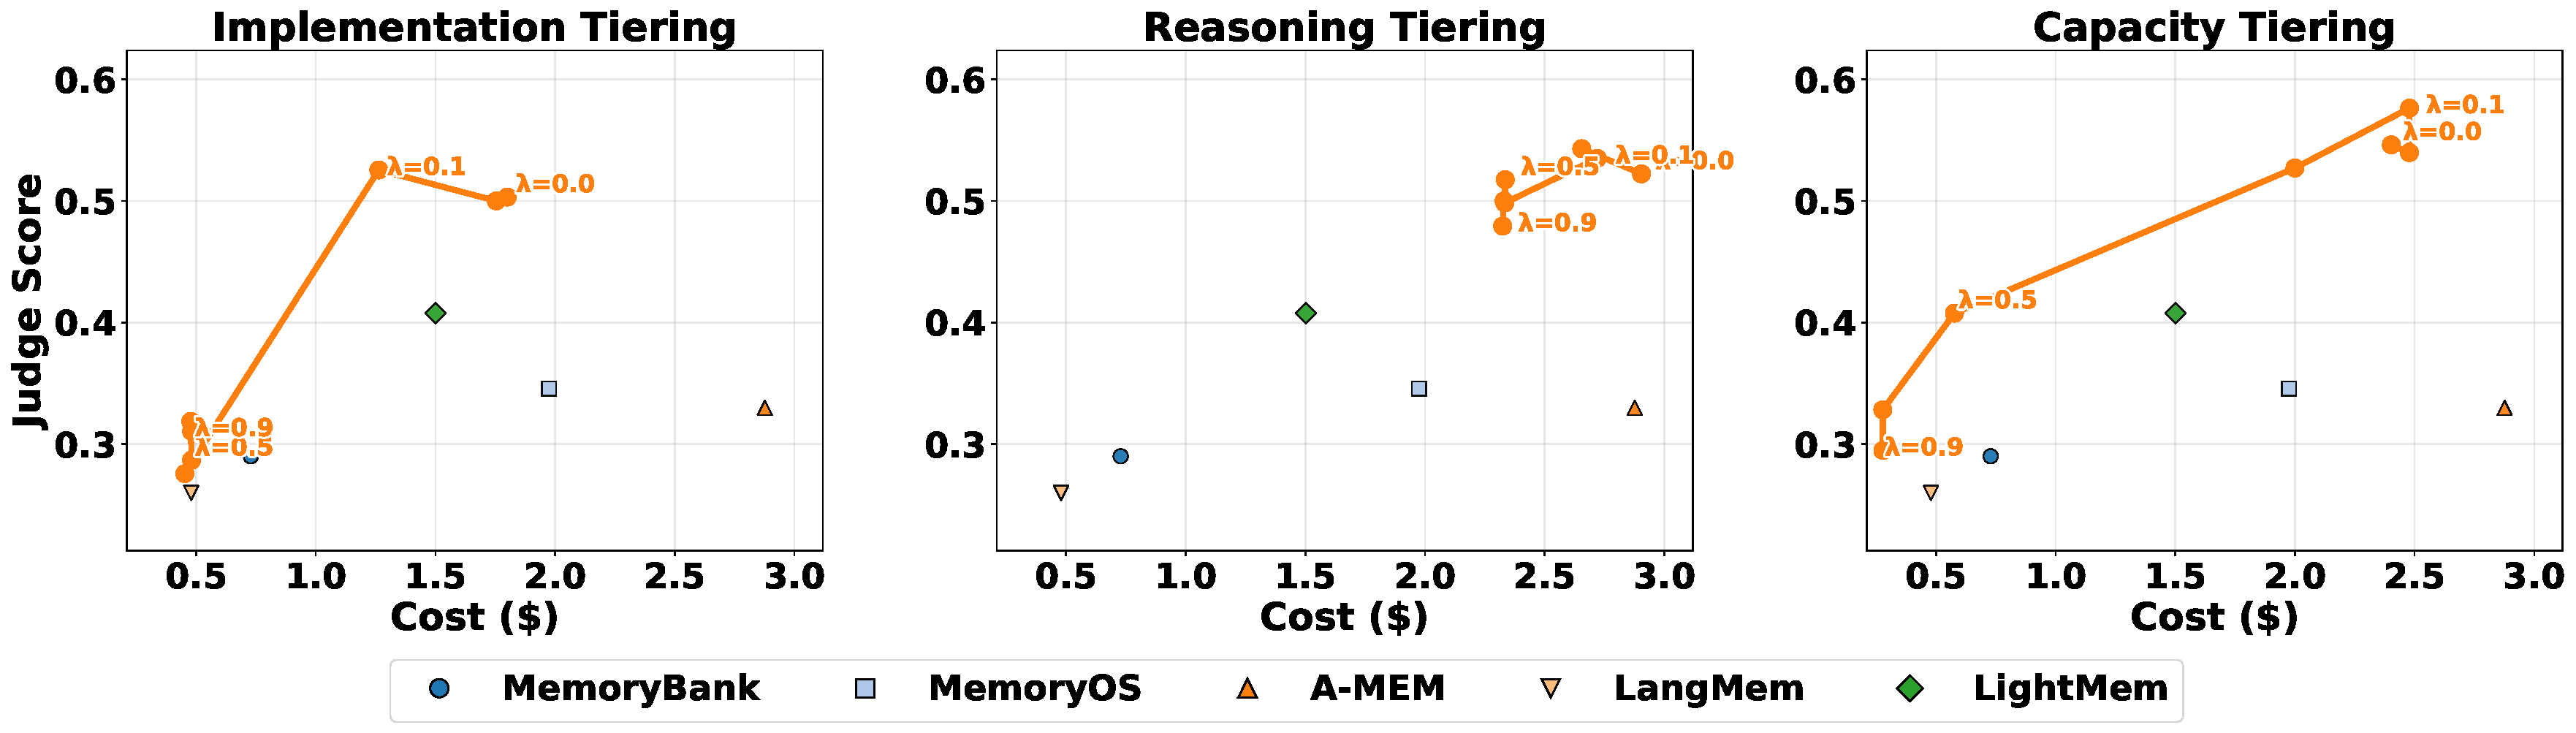
\includegraphics[width=1.0\linewidth]{figs/locomo_strategy_ABC.pdf}
        \caption{\textbf{LoCoMo 上不同分层策略的性能--成本权衡。}通过改变成本权重 $\lambda$，BudgetMem 描绘出平滑、可控的前沿；随着预算增加，该前沿向更高性能移动，并在低成本和高成本区间均包络基线。}
	\label{Trade_off_Across_Tiering_Strategies}
\end{figure*}

\section{实验分析}
\label{sec:exp_analysis}

实验组织如下。
第~\ref{sec:main_results} 节报告性能优先设置（$\lambda=0$）的结果，并比较三个变体：\textbf{BudgetMem-\textsc{Imp}}、\textbf{BudgetMem-\textsc{Rea}} 和 \textbf{BudgetMem-\textsc{Cap}}。
第~\ref{sec:trade-off} 节通过改变 $\lambda$ 描绘性能--成本曲线；第~\ref{sec:ablation} 节消融成本建模与奖励设计；第~\ref{sec:discussion} 节给出进一步分析。

\subsection{主要结果}
\label{sec:main_results}

如表~\ref{tab:exp_main} 所示，我们在性能优先设置下，于 LoCoMo、LongMemEval 和 HotpotQA 上评估 BudgetMem，并与多种代表性记忆系统进行比较。
结果支持以下三个关键发现。

\textbf{有效性。}
BudgetMem 在三个数据集上都取得显著提升，并在 F1 和 LLM 评审两项指标上持续优于既有方法。
例如，在采用 LLaMA-3.3-70B 骨架的 LongMemEval 上，BudgetMem-\textsc{Cap} 的评审分数达到 60.50，大幅超过最强基线 LightMem 的 48.51，说明其利用长上下文证据的能力更强，答案质量也更高。

\textbf{在可控成本下取得强劲性能。}
即使在性能优先区间，BudgetMem 仍具有较高成本效率，能够在不产生过量开销的情况下提升质量。
尤其是在使用 Qwen3-Next-80B-A3B 的 HotpotQA 上，BudgetMem-\textsc{Cap} 以 0.22 的成本取得最佳评审分数 72.08；BudgetMem-\textsc{Rea} 则以更低的 0.17 成本取得接近的 70.83。
这种效率源于 BudgetMem 的运行时按需设计：它不在离线阶段处理全部历史，而是检索与查询相关的原始文本块，并且只在需要时投入抽取计算。
LoCoMo 是一个例外：该数据集的历史较短，离线流水线产生的开销也较小，因此不同方法之间的成本差异不那么明显。

\textbf{汇总结果上的整体性能最强。}
汇总各数据集的结果后，BudgetMem 各变体在每个骨架模型分组中都稳定名列前茅，说明其整体有效性很强，增益并非局限于单个基准。
该趋势在 LLaMA 和 Qwen 上均成立，表明在性能优先区间内，BudgetMem 能在多样的评估设置中普遍取得强劲表现。

\subsection{探索不同分层策略的权衡}
\label{sec:trade-off}

如图~\ref{Trade_off_Across_Tiering_Strategies} 所示，我们系统比较了 LoCoMo 上三个分层维度的性能--成本分布。
随着预算约束放宽，即 $\lambda$ 减小，BudgetMem 在成本--性能平面上呈现平滑的左上移动趋势，形成连续且可控的权衡前沿。
该前沿在低成本与高成本区间均包络既有基线，能够在相近成本下取得更高评审分数，或在相近性能下实现更低成本。

值得注意的是，\emph{实现分层}与\emph{容量分层}覆盖了更宽的成本范围：实现分层在中等预算下迅速提高评审分数；随着预算增加，容量分层继续把前沿向外推进，并在高预算区间取得最佳质量。
相比之下，\emph{推理分层}呈现明显的成本集中现象。
其主要调整推理行为，例如直接生成与反思，同时保持底层模型容量不变，因此额外成本主要来自相对稳定的词元开销，成本分布范围更窄。
这一模式表明，推理维度更像是在有限成本带宽内工作的细粒度质量旋钮：它能以相近成本带来有意义的改进，但相比实现分层和容量分层，不太适合探索极低预算设置，也难以外推至极高预算性能。
总体而言，从预算受限到性能优先区间，BudgetMem 始终推动帕累托前沿向外移动。
不同分层维度之间的差异进一步表明，实现分层和容量分层更适合扩大预算覆盖范围并外推性能边界，而推理分层最适合在成本相对集中的区域内精细提升质量。

\subsection{奖励尺度对齐消融}
\label{sec:ablation}

如图~\ref{Ablating_of_Reward_Scaling} 所示，我们在 LoCoMo 上采用容量分层策略，对奖励尺度对齐（第~\ref{sec:learn_routing} 节）进行消融。
任务奖励与成本奖励在尺度和波动性上可能存在显著差异，因此移除对齐会使优化不稳定，并可能使学习偏向成本项，最终得到退化的低成本策略。
实验上，在不进行奖励尺度对齐且成本权重 $\lambda{=}0.3$ 时，路由器坍缩为对大多数模块选择 \textsc{低}档，答案质量显著下降，评审分数也降至最低。
相比之下，启用奖励尺度对齐后，路由器学会更有层次地使用不同档位，产生平滑得多、行为也更合理的性能--成本前沿。
该消融说明，奖励尺度对齐对于平衡学习信号十分重要；它使系统实现有意义的成本--性能控制，而不是退化为简单的成本最小化。

\begin{figure}[h]
	\centering
	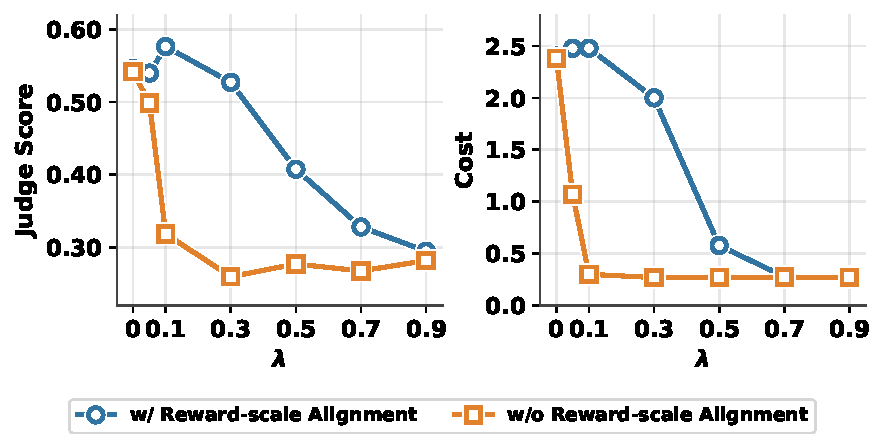
\includegraphics[width=1.0\linewidth]{figs/ablation_cost_reward_scaling.pdf}
        \caption{\textbf{奖励尺度对齐消融。}在 LoCoMo 上采用容量分层策略。}
	\label{Ablating_of_Reward_Scaling}
\end{figure}

\subsection{讨论}
\label{sec:discussion}

\paragraph{预算档位选择比例。}
图~\ref{Module_Ratio} 采用容量分层策略，通过报告不同成本权重 $\lambda$ 下 \textsc{低}/\textsc{中}/\textsc{高}档位的选择比例，分析 LongMemEval 上的模块级路由行为。
总体而言，路由器呈现出清晰、可解释的预算响应：随着成本压力增大，它系统地把概率质量从高成本档位转移至更便宜的档位，从模块层面证明 BudgetMem 会以成本感知方式分配计算。

更具体地说，当 $\lambda$ 较小，例如 0.1 时，路由器把大多数模块分配到 \textsc{中}档，优先保证质量。
当 $\lambda=0.3$ 时，它在保留可观 \textsc{中}档比例的同时提高 \textsc{低}档占比，体现出对计算量的可控削减。
在更大的 $\lambda$ 下，为满足更严格的成本偏好，策略进一步在各模块上集中选择 \textsc{低}档。
总体来看，这些趋势证实 BudgetMem 会随着预算偏好变化，以可预测的方式调节不同档位的使用。

\begin{figure}[h]
	\centering
	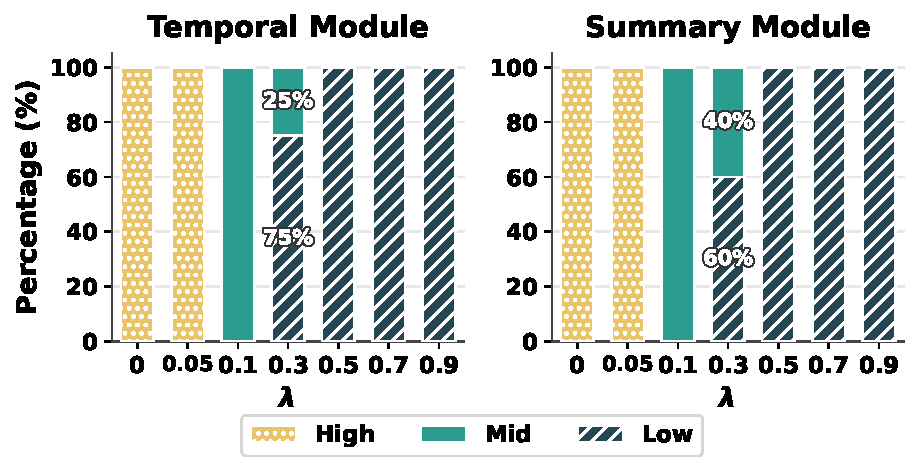
\includegraphics[width=1.0\linewidth]{figs/strategy_c_ratio_comparison.pdf}
        \caption{\textbf{预算档位选择比例。}采用容量分层策略时，LongMemEval 上不同成本权重 $\lambda$ 所对应的模块级 \textsc{低}/\textsc{中}/\textsc{高}路由比例。}
	\label{Module_Ratio}
\end{figure}

\paragraph{检索规模敏感性分析。}
图~\ref{sensitivity_analysis} 展示了在三种分层策略下，改变 LoCoMo 上检索原始文本块数量时的成本和评审分数。
由于输入更长且需要额外处理，增加检索规模会如预期般提高成本；更多支持证据也往往会提高评审分数，这体现了证据覆盖范围与计算开销之间的标准权衡。

然而，收益并非单调增长。
在我们的设置中，检索 5 个文本块能在成本与质量之间取得最佳平衡。
检索过多文本块可能降低性能：额外文本块会引入更多冗余或弱相关内容，增加噪声并可能分散 LLM 的注意力，从而降低评审分数。
反之，检索块过少会导致证据不足，限制下游增益。
总体而言，这些结果表明，检索规模是一个重要的实用控制旋钮，可在证据充分性、上下文噪声与成本之间取得平衡。

\begin{figure}[h]
	\centering
	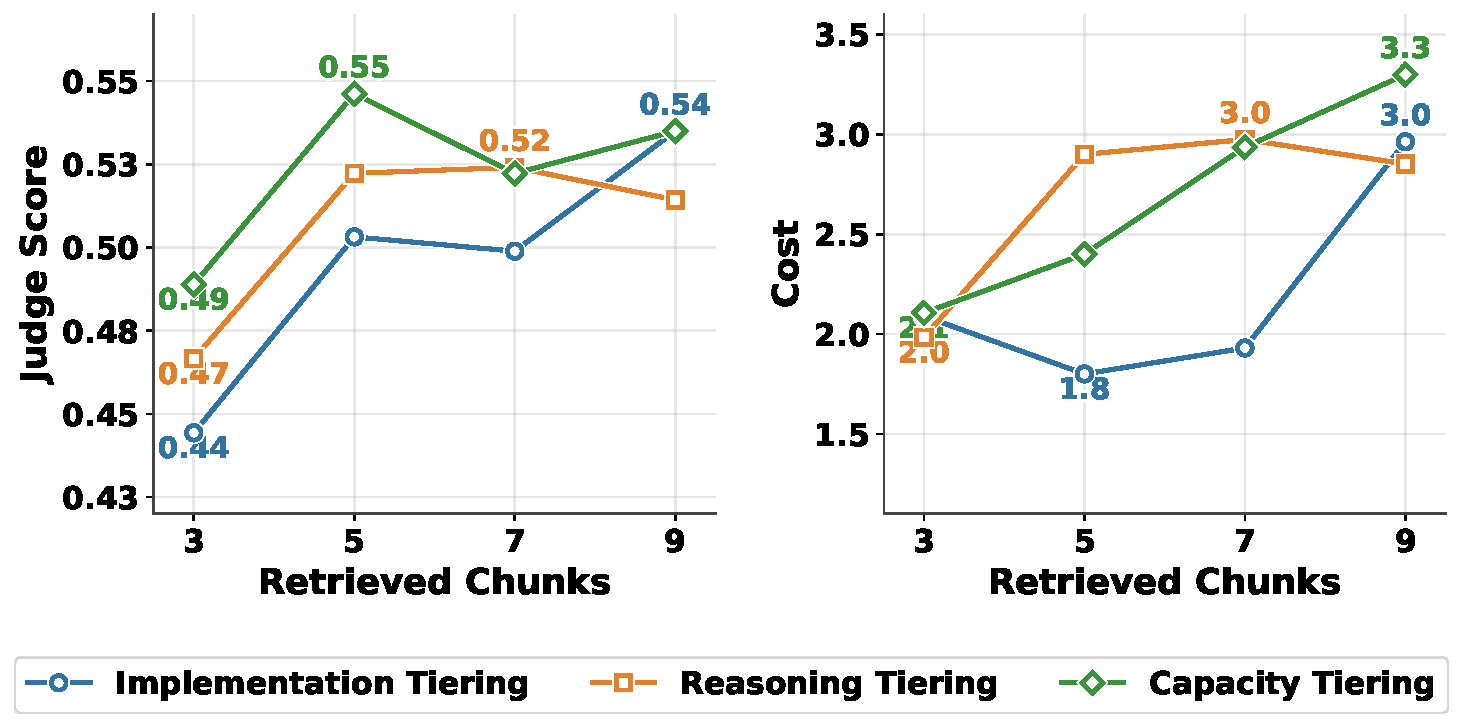
\includegraphics[width=1.0\linewidth]{figs/sensitivity_analysis.pdf}
        \caption{\textbf{LoCoMo 上的检索规模敏感性。}在三种分层策略下，成本和评审分数随检索原始文本块数量的变化。}
	\label{sensitivity_analysis}
    \vskip -0.1in
\end{figure}

\paragraph{延迟分析。}
尽管我们的主要成本指标聚焦货币成本，延迟对于实际部署同样重要。
因此，我们在受控的本地部署中额外测量延迟：所有方法共享 Qwen 骨架，并采用相同的硬件与推理栈。
该比较不使用 API 延迟，因为网络状况与服务提供方调度会对其产生显著影响，不适合进行公平的相对比较。
表~\ref{tab:latency_locomo_detail} 和表~\ref{tab:latency_locomo_batch} 报告该设置下的绝对延迟；我们主要利用它们比较不同方法的相对流水线开销。

如表~\ref{tab:latency_locomo_detail} 所示，在不同预算设置下，BudgetMem 呈现出预期的延迟权衡。
对于实现分层，提高成本权重会把总推理延迟从 $\lambda=0$ 时的 3881 毫秒降至 $\lambda=0.9$ 时的 1167 毫秒，同时检索/过滤延迟从 1176 毫秒降至 46 毫秒。
推理分层与容量分层也会降低延迟，但降幅较小，因为其档位主要改变推理行为或模型容量，而不是替换过滤实现。
此外，测得的 GPU 时间始终较短，每个查询约为 44--52 毫秒，说明轻量级路由器自身引入的开销有限。
如表~\ref{tab:latency_locomo_batch} 所示，所有方法均能从批处理中受益，且 BudgetMem 的相对开销在不同服务设置下大体一致。
总体而言，这些结果说明检索/过滤开销在实践中是可控的；对完整流水线进行系统级加速与本文目标正交，留待未来工作研究。

\begin{table}[h]
    \centering
    \footnotesize
    % \setlength{\tabcolsep}{2.5pt}
    \caption{\textbf{受控本地部署下 LoCoMo 的详细延迟。}
    批大小为 1，所有数值的单位均为毫秒。
    \textbf{离线}表示平均离线记忆构建时间，
    \textbf{总计}表示平均总推理延迟，
    \textbf{过滤}表示平均检索/过滤模块延迟，
    \textbf{GPU} 表示平均 GPU 时间。
    N/A 表示不适用或未测量。}
    \label{tab:latency_locomo_detail}
    \begin{tabular}{@{}lrrrr@{}}
        \toprule
        \textbf{方法} & \textbf{离线} & \textbf{总计} & \textbf{过滤} & \textbf{GPU} \\
        \midrule
        MemoryOS & 40657 & 2842 & 1488 & N/A \\
        A-MEM    & 26842 & 1449 & 49   & N/A \\
        LightMem & 9740  & 1662 & 62   & N/A \\
        \midrule
        本文-IMP ($\lambda=0$)   & N/A & 3881 & 1176 & 46 \\
        本文-IMP ($\lambda=0.3$) & N/A & 2432 & 556  & 46 \\
        本文-IMP ($\lambda=0.9$) & N/A & 1167 & 46   & 46 \\
        \midrule
        本文-REA ($\lambda=0$)   & N/A & 3678 & 1274 & 47 \\
        本文-REA ($\lambda=0.3$) & N/A & 3429 & 1216 & 45 \\
        本文-REA ($\lambda=0.9$) & N/A & 3318 & 1209 & 48 \\
        \midrule
        本文-CAP ($\lambda=0$)   & N/A & 3461 & 1228 & 44 \\
        本文-CAP ($\lambda=0.3$) & N/A & 3058 & 1079 & 46 \\
        本文-CAP ($\lambda=0.9$) & N/A & 2853 & 976  & 52 \\
        \bottomrule
    \end{tabular}
\end{table}


\begin{table}[h]
    \centering
    \footnotesize
    % \setlength{\tabcolsep}{3pt}
    \caption{\textbf{LoCoMo 上的批大小扩展。}
    我们报告不同批大小下的平均总推理延迟，所有数值单位均为毫秒。
    \textbf{BS} 表示批大小。
    BudgetMem 报告 $\lambda=0$ 的本文-REA。}
    \label{tab:latency_locomo_batch}
    \begin{tabular}{@{}lrrrr@{}}
        \toprule
        \textbf{BS} & \textbf{MemoryOS} & \textbf{A-MEM} & \textbf{LightMem} & \textbf{本文-REA} \\
        \midrule
        1  & 2842 & 1449 & 1662 & 3678 \\
        2  & 1633 & 845  & 1059 & 2295 \\
        4  & 974  & 518  & 775  & 1327 \\
        8  & 604  & 296  & 438  & 858  \\
        16 & 387  & 154  & 269  & 547  \\
        32 & 203  & 96   & 163  & 326  \\
        \bottomrule
    \end{tabular}
\end{table}

